\documentclass[11pt]{article}
\usepackage[margin=0.6in]{geometry}
\usepackage[utf8]{inputenc}
\usepackage{authblk}
\usepackage{doi}
\usepackage{tcolorbox}
\usepackage{enumitem}
\usepackage{graphicx,pdflscape,multirow}
\usepackage{array}
\usepackage{xcolor}
\usepackage{multicol}
\usepackage{wrapfig,lipsum,booktabs}
\usepackage{fancybox}
\usepackage{amsmath}

\newcommand{\fixme}[1]{{\color{red} (#1)}}
\newcommand{\coloc}{\texttt{escheR}}

% \renewcommand\Authfont{\fontsize{8}{14.4}\selectfont} % change author fontsize
% \renewcommand\Affilfont{\fontsize{6}{10.8}\itshape}   % change auth affil fontsize
\makeatletter % make affiliations on one line
\renewcommand\AB@affilsepx{, \protect\Affilfont}
\makeatother

\usepackage[sort&compress,square,numbers]{natbib}
\bibliographystyle{unsrtnat}

%\setmainfont{Helvetica}
\title{\coloc: Optimize Spatial Visualization Following Gestalt Principles}
\author[1]{Boyi Guo\thanks{Corresponding author}}
\author[1]{Stephanie C. Hicks}
\affil[1]{Department of Biostatistics, Johns Hopkins Bloomberg School of Public Health, MD, USA}
\date{\today}

\begin{document}
\maketitle

\vspace{-.6in}

%% ABSTRACT ============================================================================================
\section*{Abstract}
\subsection*{Summary}
Colocalization is highly interested research questions in the analysis of spatial omics data. While many sophisticated computational models are proposed to infer the colocalization relationship between genes or proteins in the spatial context, there completely lack of intuitive spatial visualization, making interpretation extremely challenging. The biggest challenge for colocalization visualization is two sources of orthogonal information, spot colocalization and spot membership (such as spatial domain) the same spatial plot. To address this issue, we developed \coloc to display the colocalization while maintaining an intuitive representation of the surrounding spatial domain. \coloc leverages color contrast optical illusion to display spatial domains to create shadows representing different spatial domain while using different spots to denote colocalization status.  

\subsection*{Availability and implementation}
The R package \coloc is freely available at Github (\url{https://github.com/boyiguo1/VisColoc}).
% and Zenodo (\fixme{add link}).


%% INTRODUCTION ============================================================================================
\section*{Introduction}
Visualization is an indispensable component of data analysis, providing clarity that connects quantitative evidence to key conclusions. \cite{dagostinomcgowan_2022} In bioinformatics research, visualization receives growing recognition as essential: many scientists rely on visualization to complete their cognitive process from analysis to insight, including analytic validation of automated pipelines and scientific communication. \cite{odonoghue_2021} Nevertheless, current methods and tools are inadequate to visualize the growingly complex biological data and computational models, limiting the ability to derive new insights and discoveries. \cite{odonoghue_2010}  

The recent technology breakthrough in spatial profiling enables characterizing the diversity of molecules, e.g. DNA, RNA, and proteins, in the spatial context \cite{moffitt_2022}, generating novel spatially-resolved data that requires highly tailored \textit{in situ} visualizations \cite{dries_2021, Lewis_2021, odonoghue_2021}. Current \textit{in situ} visualizations, as opposed to embedding visualizations (e.g. t-SNE and UMAP) that project information to some mathematical space, visualize molecular information in the original cellular location, creating spatial maps that color-code a single variable (e.g., molecule expression, cell type, or spatial domain). This approach lacks the ability to simultaneously exhibit multiple variables, possibly from disparate data domains (such as expression domain and spatial domain) or modalities (such as transcriptomics and proteomics), creating cognitive gaps to interpret findings regarding their (micro-) environment. For example, when studying differential expression in different spatial domains (commonly defined by tissue architecture, e.g. cancerous regions, cortical layers), two spatial maps are displayed side-by-side, one for gene expression and one for spatial domains, creating significant challenges to associate these two information together. While software-based interactive visualizations or 3-D visualizations have the potential to mitigate this challenge, they are infeasible for scientific communications in static media, such as prints. Developing a static spatial visualization that enables the simultaneous display of multiple dimensions of information is crucial for spatially-resolved data research.

% Previous data visualization of omics largely relies on projecting the omics space to an embedding space, such as t-SNE and UMAP, which is infeasible for spatial omics technologies.

 To optimize \textit{in situ} visualization, we introduce gestalt principles to the design of spatial maps. Gestalt principles \cite{todorovic_2008, palmer_1999} refer to a set of rules describing how humans perceive and interpret visual information and are commonly applied in art and designs. Following gestalt principles, we add additional visual dimensions to spatial maps, leveraging different aesthetics, such as color, fill, and symbols, to simultaneously display disparate variables. Specifically, we apply figure-ground articulation to display two variables: one variable (e.g. expression) can be plotted as color-filled circles, serving as the \textit{figure}; one variable (e.g. spatial domains) can be plotted as the backgrounds of the circles, creating a \textit{ground} for the figure. For adjacent circles with limited space between them to display the background color, we use an economic implementation, colored outlines for these circles, inspired by watercolor effect \cite{pinna_1987, pinna_2001}. Watercolor effect describes the phenomenon in visual perception that surface color arises from thin boundaries and hence is applied here to perceive the background color in tight space. Overall, the figure-ground articulation creates two isolated layers in visual perception to display the two variables while maintaining the relative spatial relationship serving as a reference between the two. In addition, other fundamental principles \cite{todorovic_2008}, such as proximity, similarity, continuity, and closure, incentivize the brain to group elements and dimensions in the visualization, guaranteeing an integrative perception of the complex multi-dimensional spatial map.
 

The main thrust of \coloc is to integrate another dimension of information to the spatial map using color contrast optical illusion. The color contrast optical illusion is a phenomenon where the appearance of a color is influenced by the colors surrounding it. This illusion occurs due to the way our brain processes visual information and perceives color. In a spatial map, we can construct each spatial unit as a hollow point using \texttt{ggplot2::geom\_points} where the boundary of each spatial unit are color-coded to represent one dimension of the information, working for both continuous measures such as gene expression or categorical measures such as spatial domains. It is possible to add another layer of information for an additional variable using symbols or contrast colors on side of each spot. Hence, within each spatial map, multiple layers of information can be displayed jointly.

\coloc is  an open-source package implemented in the R programming environment. The package \coloc is constructed based on \texttt{ggplot2} and can be easily integrated into any spatial visualization pipeline, for example, \texttt{spaitalLIBD} and \texttt{seurat}, that adapts \texttt{ggplot2} principles and would be able to generalize to users in both Bioconductor community and seurat community
 
 in an interactive process
 
 We provide an R package called \coloc (named after the graphic artist M.C. Escher) to implement this visual innovation. 
 
 
 , following an iterative process that adds layers to a spatial map. Extending \texttt{ggplot2}, \coloc can seamlessly integrate to any established visualizations that is based on the most popular R visualization framework \texttt{ggplot2}, following the same syntax. We apply \coloc to the spatial transcriptomics dataset (Fig. 1G). The results show \fixme{colocalization}.



\section*{Use Case 1: Differential Expression in Spatial Domains}
To demonstrate the new visualization, we apply \coloc to visualize the colocalization of two genes, (FYN) and (EFNA5) in the human dorsolateral prefrontal cortex. The two genes are previously identified that relates to SCZ expression via cell-cell communication analysis. The purpose of the visualization is to see if the density of colocalization are different across different cortex layers. Using \coloc, we can simultaneously display the colocalization and cortex layer in the same spatial plot, instead of having two saprate plots, one for cortex layer and one for colocalization, making the verification of the visual within the spaital context more straightforward and easier. 

To create a colocalization plots, \coloc follows a similar principle as \texttt{ggplot2}'s layering strategy. In the first step, we will use the funciton \texttt{spCOCOON} to create a base plot that converts a spatial transcroptimcs data structure to a plot object. In a second step, we use the function \texttt{add\_fill} to color code each spots with colcalization status, which includes three levels, spots that expressed both genes and spots that expressed either of the genes. Then, we will apply the function \texttt{add\_COCOON} to show the spatial domain (cortex layer) information. Optionally, one can apply the funciton \texttt{add\_symbol} to display another layer of information. Here, we use  the symbol to highlight the colocalization spots, i.e. the spots that expresses both genes. Because we followed the layering strategy that \texttt{ggplot2}. One can seamsely to integrate \coloc to any \texttt{ggplot2}-based spatial visiulization by piping a \texttt{ggplot2} object to \texttt{add\_COCOON} and \texttt{add\_symbol} and customize the plots using the \texttt{ggplot2} syntex and themes, greatly reduce the techinical burden to customize these new spatial plot designs.  

\section*{Use Case 2: Multi-dimensional UMAP Plot}


\section*{Summary}

While \coloc is to design to display colocalization in their spatial context, the underlying principle can be broadly applied to address visualizaiton challenges in informaiton rich visualizations. The contrast color optical illusion provides allows to add another dimension of information in any spatial visualization, which can be further used to display multi-omics presence, greatly improve the interpretability. 

In this manuscript, we demonstrate the utility of the proposed spatial visualization using spot-based spatial resolved data, nevertheless, this method can be applied to image-based spatial resolved data by applying \texttt{schex} to avoid overplotting commonly for image-based spatial resolved data, similar to our second UMAP example where the first step is to reduce done the dimensiona

our programming provides flexibility by following the grammar of graphs, especially ggplot2


translating the findings in vision science to dat science to address many of the current challenges in visualization.


%% EPILOGUE ================================================================
\section*{Acknowledgements}
B.G. would like to acknowledge Dr. Leonardo Collado Torres,  and Louise Huuki-Myers for their helpful feedback.

\vspace{0.2in}
\noindent \textit{Conflict of Interest:} none declared.

\section*{Data availability}
The spatial transcriptomics dataset was obtained from \texttt{spatialLIBD}(\url{http://research.libd.org/spatialLIBD/}). The code that generates these figures are deposited at \fixme{github manuscript repo}.

\clearpage
% \vspace{-0.1in}
\begin{wrapfigure}[13]{r}{0.8\textwidth}
\vspace{-0.3in}
\begin{center}
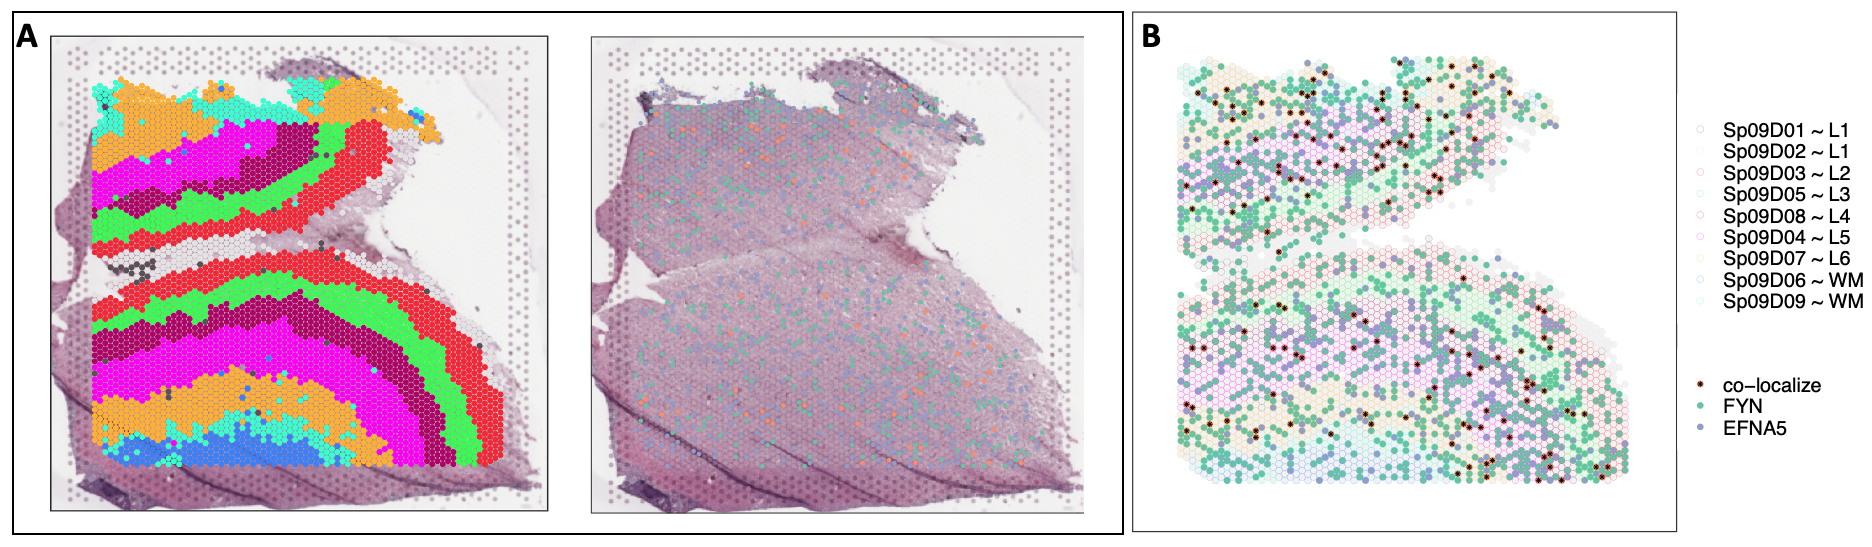
\includegraphics[width=0.78\textwidth]{figure/new_visiual.png}
\end{center}
\vspace{-0.35in}
\caption{\footnotesize \textbf{Optimized visualization interpreting co-localization in the spatial context}. (\textbf{A}) Current visualization of co-localization requires two separate plots, one to display spatial domain information and one to display co-localization, difficulty to associate the two sources of information for interpretation. (\textbf{B}) The proposed visualization is optimized to display both spatial domain and co-localization information in one plot.}
\label{fig:visual} 
\end{wrapfigure}

%% BIBLIOGRAPHY ==========================================================

\clearpage 
% \printbibliography
\bibliography{refs}

\end{document}


